\subsection{7 Sites Results}

We'd like to isolate out the impact of simply resource pooling. Thus
it makes sense to conduct experiment on the case where instead of
having some big sites and small sites, we have 7 small sites, each
with one machine. This system has worse performance to begin with
because no pooling effect is present initially. Let's look at the
impact of diversions.

\begin{figure}[htp]
\centering
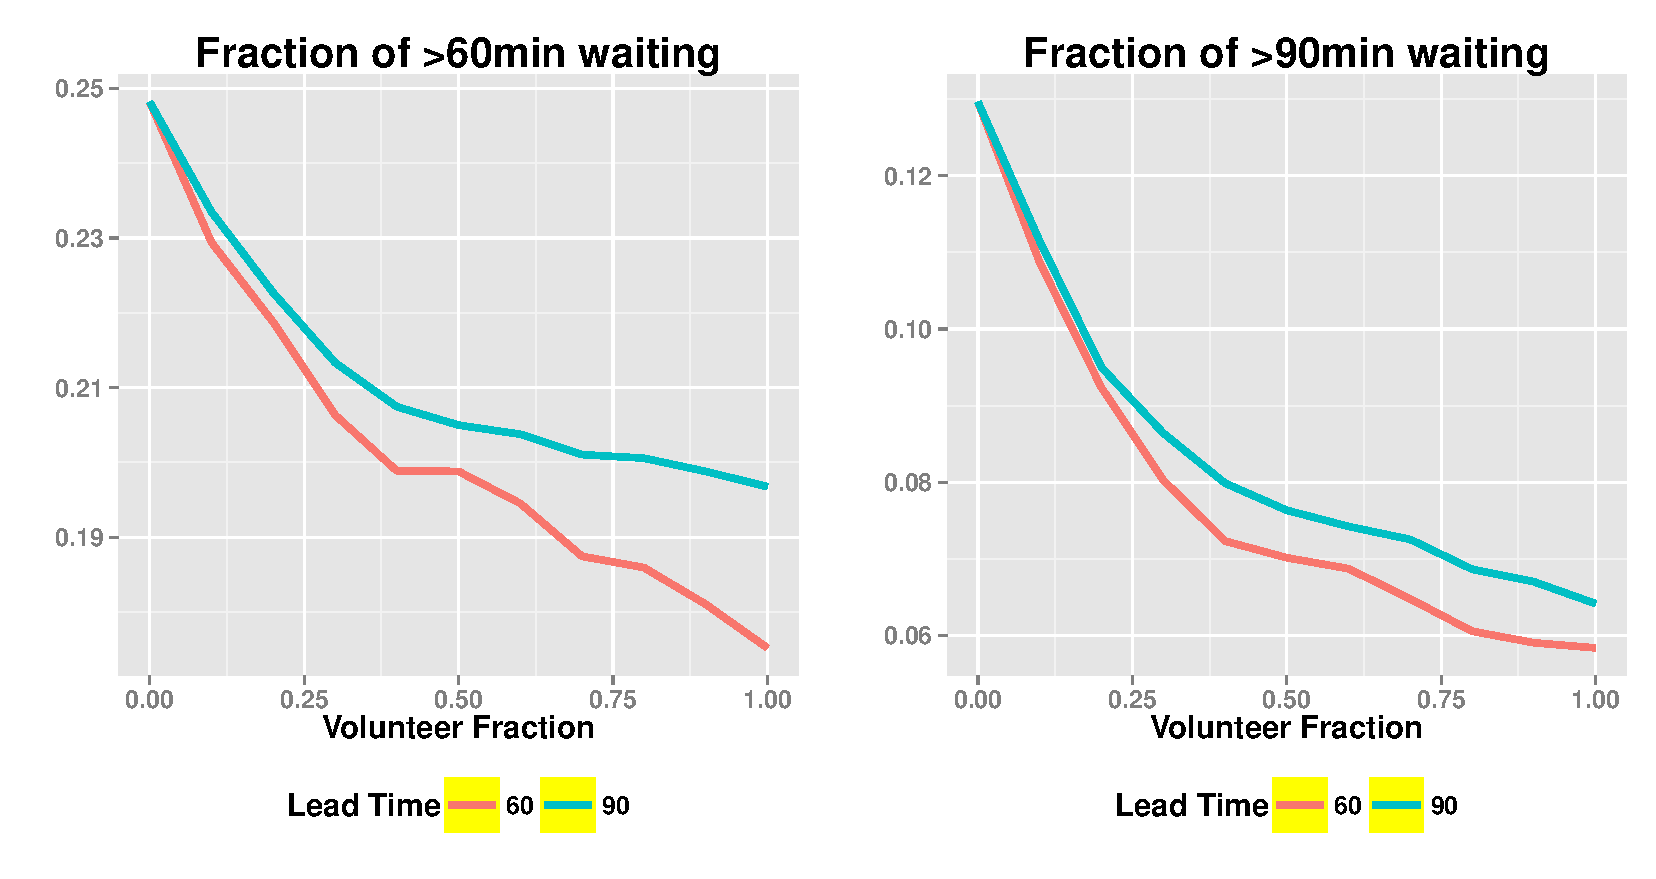
\includegraphics[width=.9\textwidth]{chap3/numeric/pic/7sites_extreme}
\caption{The impact on extreme waiting by diversions. Compare to
3 sites case, we much more significant improvement.}
\label{fig:7sites_extreme}
\end{figure}

\begin{figure}[htp]
\centering
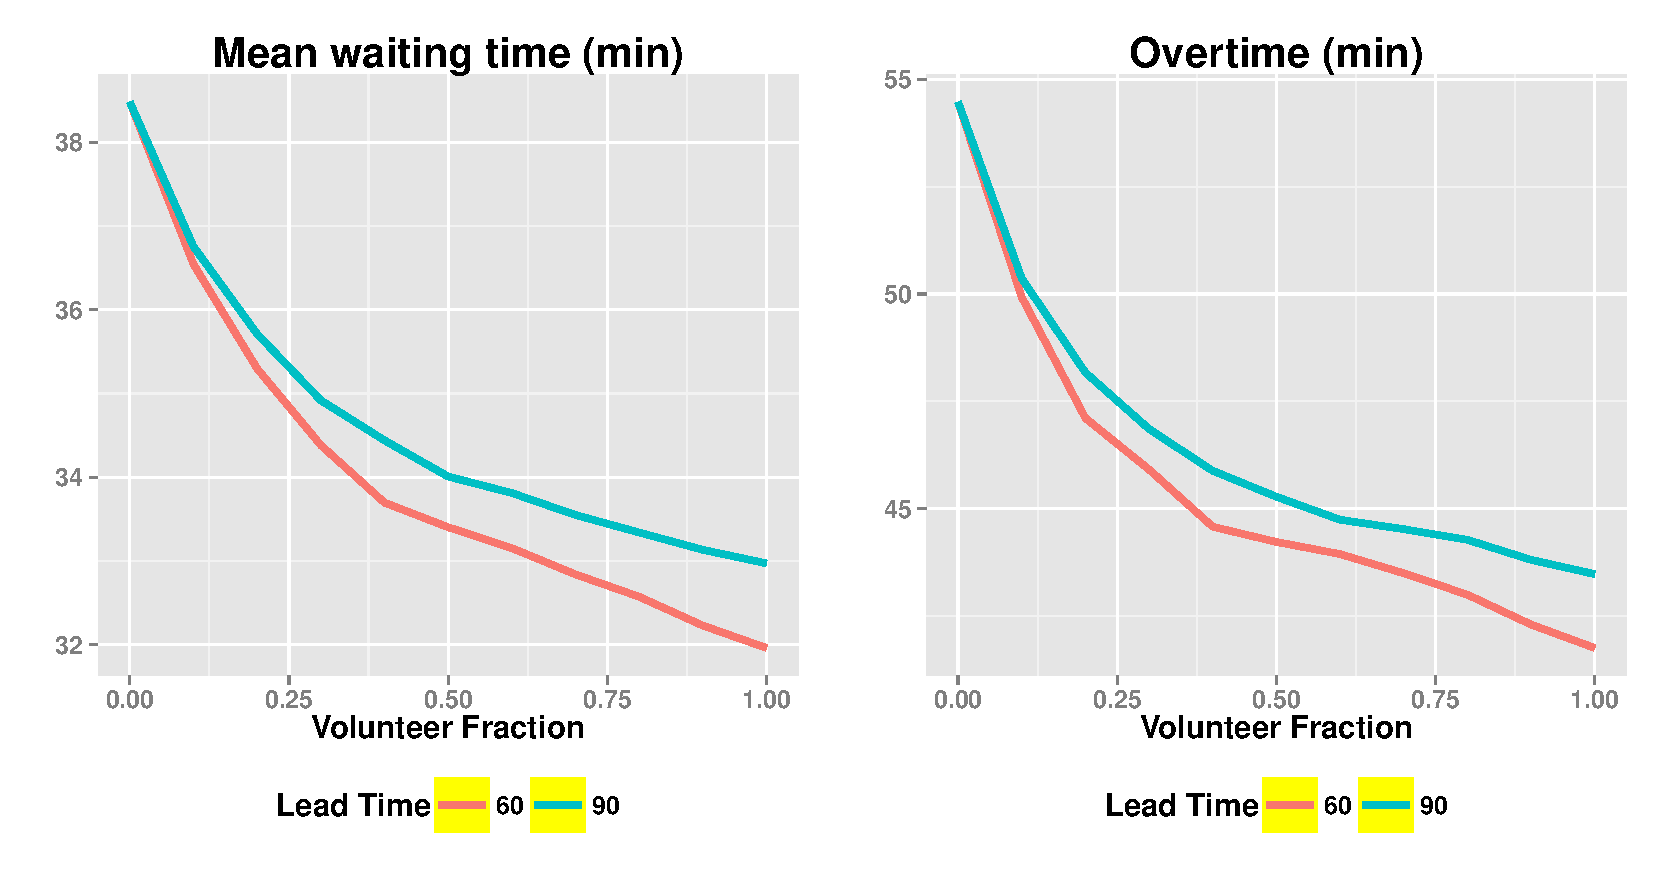
\includegraphics[width=.9\textwidth]{chap3/numeric/pic/7sites_wait_overtime}
\caption{The impact on mean waiting time and overtime by diversions.}
\label{fig:7sites_wait_overtime}
\end{figure}

Figure \ref{fig:7sites_extreme} shows that we have more significant
improvement compared to 3 sites case. This confirmed our intuition
that bigger improvement can be achieved with no pooling effect to begin with.
Figure \ref{fig:7sites_wait_overcome} tells the same story for mean
waiting time and overtime. Note in the end, we can improve mean waiting
time from 38min to 30min, with a 8min difference. And the story is
similar for overtime.

\begin{figure}[htp]
\centering
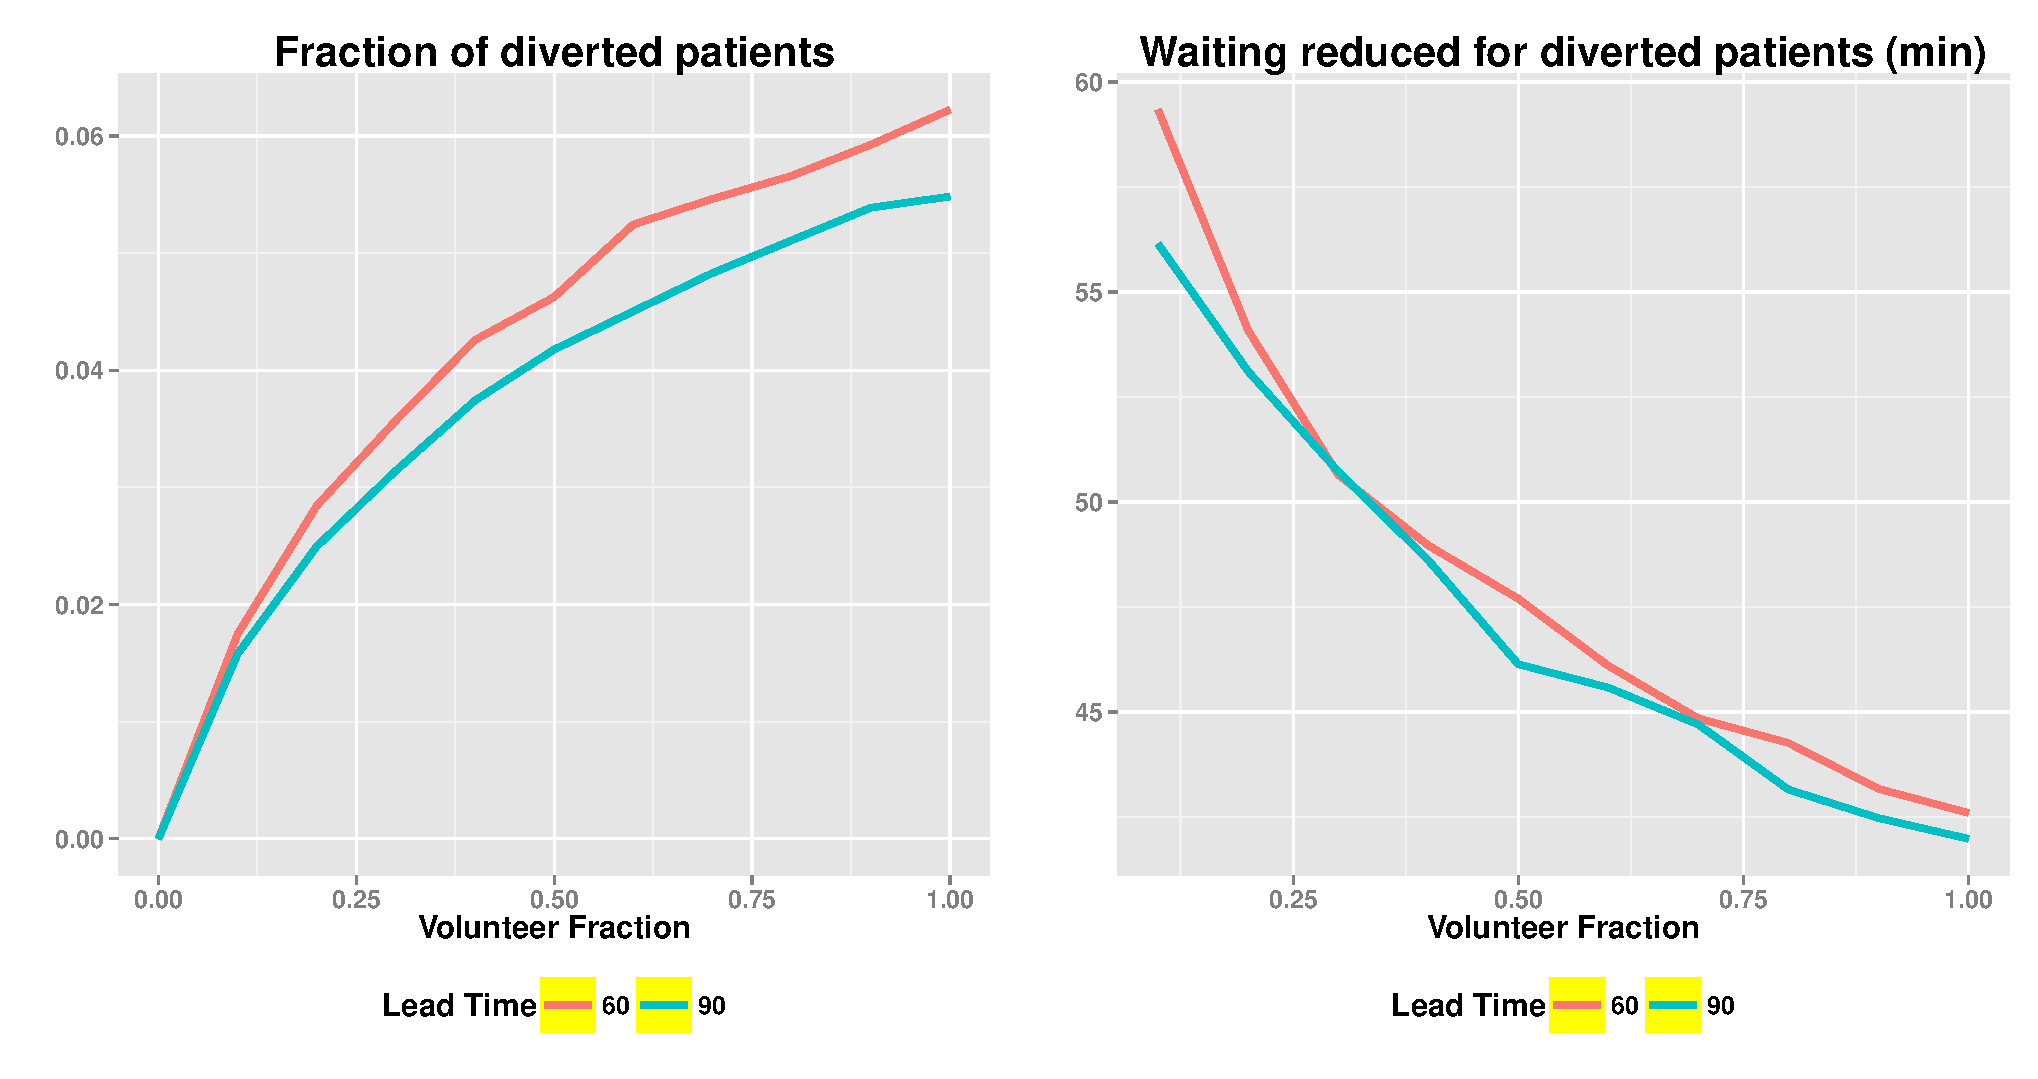
\includegraphics[width=.9\textwidth]{chap3/numeric/pic/7sites_diversion_gain}
\caption{The fraction of diversions and waiting time reduction from diversions.}
\label{fig:7sites_diversion_gain}
\end{figure}

From Figure \ref{fig:7sites_diversion_gain}, we see that we diverted a lot
more patients compared to 3 sites case. With all patients as volunteer, we
diverted more than 6\% of them. This shows that there are a lot more
beneficial diversion opportunities when there is no initially. Also, for
diverted patients, each of them also enjoys more waiting time reduction
compared to 3 sites case.

Note that here all 7 sites are totally homogeneous so there won't be any
unbalance in term of diversion flow and all improvement is equally achieved
by all sites.

Overall, the experiments for the 7 site confirms that greater benefit can
be achieved in the system with many small sites.
